
%%% LaTeX Template: Article/Thesis/etc. with colored headings and special fonts
%%%
%%% Source: http://www.howtotex.com/
%%% Feel free to distribute this template, but please keep to referal to http://www.howtotex.com/ here.
%%% February 2011
%%%
%%% Modified October 2015 by CDM

%%%  Preamble
\documentclass[11pt,letterpaper]{article}
\usepackage[margin=1.0in]{geometry}
\usepackage[T1]{fontenc}
\usepackage[bitstream-charter]{mathdesign}
\usepackage[latin1]{inputenc}					
\usepackage{amsmath}						
\usepackage{xcolor}
\usepackage{cite}
\usepackage{hyphenat}
\usepackage{graphicx}
\usepackage{float}
\usepackage{subfigure}
\usepackage{sectsty}
\usepackage[compact]{titlesec} 
\usepackage[tablegrid]{vhistory}
\allsectionsfont{\color{accentcolor}\scshape\selectfont}

%%% Definitions
\definecolor{accentcolor}{rgb}{0.0,0.0,0.5} 
\newcommand{\teamname}{TrafficNetPeons}
\newcommand{\productname}{Product Name: TBD}
\newcommand{\coursename}{CSE 4316: Senior Design I}
\newcommand{\semester}{Fall 2016}
\newcommand{\docname}{Project Charter}
\newcommand{\department}{Department of Computer Science \& Engineering}
\newcommand{\university}{The University of Texas at Arlington}
\newcommand{\authors}{Peyton Casper \\ Ruchitha Thalakola \\ Jose Hernandez \\ Rabin Dhoubanjar \\ Kyle Edelmann}

%%% Headers and footers
\usepackage{fancyhdr}
	\pagestyle{fancy}						% Enabling the custom headers/footers
\usepackage{lastpage}	
	% Header (empty)
	\lhead{}
	\chead{}
	\rhead{}
	% Footer
	\lfoot{\footnotesize \teamname \ - \semester}

	\cfoot{}
	\rfoot{\footnotesize page \thepage\ of \pageref{lastpage}}	% "Page 1 of 2"
	\renewcommand{\headrulewidth}{0.0pt}
	\renewcommand{\footrulewidth}{0.4pt}

%%% Change the abstract environment
\usepackage[runin]{abstract}			% runin option for a run-in title
%\setlength\absleftindent{30pt}			% left margin
%\setlength\absrightindent{30pt}		% right margin
\abslabeldelim{\quad}	
\setlength{\abstitleskip}{-10pt}
\renewcommand{\abstractname}{}
\renewcommand{\abstracttextfont}{\color{accentcolor} \small \slshape}	% slanted text

%%% Start of the document
\begin{document}

%%% Cover sheet
{\centering \huge \color{accentcolor} \sc \textbf{\department \\ \university} \par}
\vspace{1 in}
{\centering \huge \color{accentcolor} \sc \textbf{\docname \\ \coursename \\ \semester} \par}
\vspace{0.5 in}
\begin{figure}[h!]
	\centering
   	
\includegraphics[width=0.60\textwidth]{images/test_image1
}
\end{figure}
\vspace{0.5 in}
{\centering \huge \color{accentcolor} \sc \textbf{\teamname \\ \productname} \par}
\vspace{0.5 in}
{\centering \large \sc \textbf{\authors} \par}
\newpage


%\vspace{1 in}
%\centerline{January 13th, 2012}
%\newpage

%%% Revision History
\begin{versionhistory}
  	\vhEntry{0.1}{1.19.2016}{PC|JH|RT|RD|KE}{document creation}
  	\vhEntry{0.2}{2.05.2016}{PC|JH|RT|RD|KE}{complete draft}
  	\vhEntry{0.3}{2.12.2016}{PC|JH|RT|RD|KE}{release candidate 1}
  	\vhEntry{1.0}{2.18.2016}{PC|JH|RT|RD|KE}{official release}
  	\vhEntry{1.1}{2.19.2016}{PC|JH|RT|RD|KE}{added customer change requests}
\end{versionhistory}
\newpage

%%% Table of contents
\tableofcontents
\newpage

%%% List of figures and tables (optional)
\listoffigures
%\listoftables
\newpage

%%% Agile project charter sections
\section{Vision}
TrafficNetPeons is a subsidiary of TrafficNet, LLC and therefore adheres to the mission of our parent company amenably. Within the realm of this etablished model TNP has been born from a singular ambition, to create an affordable, low power, weatherproof camera most suitable for use in the traffic monitoring industry. Thus, our vision is to provide one solution to this ambition that supports and compliments the mission of our parent company in addition to improving the general wellfare of the conventional commuter.

\section{Mission}
TrafficNetPeons, a subsidiary of TrafficNet, LLC is dedicated to making the flow of traffic safer, smarter, and simpler to manage. Our team is engaged in the development of the next generation of traffic monitoring camera modules to be mass produced and field deployed in a broad spectrum of outdoor environments to assist traffic managers and the millions of drivers on the roads each day. Through creative innovation and meticulous design, TrafficNetPeons delivers high-quality products and top-notch service. Let us help change the way you see traffic.

\section{Success Criteria}
TNP is a business founded upon integrating municipalities with their commuters. The success of our current project hinges upon providing comprehensive and secure technology to traffic monitoring officials so that they might deliver the best possible service to their communities. In further detail, to accomplish this the traffic monitoring camera we are currently engaged in the design of must be mass produced, field deployed and easily accessible only to those persons authorized in its daily usage. Only at such time when our team can confidently expect our product to be adopted by surrounding municipalities for mass use in the outdoor environment can we say we have succeeded.

\newpage

%%% Remaining project charter sections
\section{Background}
TrafficNet, LLC is a young Limited Liability Company which has made headway in the traffic monitoring industry with the BAT-433 which, uses Bluetooth technology to calculate real-time traffic analytics, including travel times, speeds, origins and destinations of local commuters. As a subsidiary of TrafficNet, TNP has accepted a role in the history of our parent company with an innovative solution to their latest ambition, the secure monitoring of even the most remote stretches of Texas highways. 


\section{Related Work}
The closest solution that exist would be the RaspberrIPCam. The RaspberrIPCam is an open source project that was built by Sons of Tone. The RaspberrIPCam streams in full HD (1080p) video streaming at 30fps, has RTSP protocol which is standard protocol for video streaming in security applications, and has web server configurations. Even though the RaspberrIPCam is close to what our project is, it stills lacks some additional features. One example would be that TrafficNet wanted the camera to have heating capabilities when bad weather was an issue, which the RaspberrIPCam does not have. Another requirement that TrafficNet wants is the camera to have a pan and tilt, which the RaspberrIPCam also does not have. Even though the RaspberrIPCam would serve as the closest solution, our team still needs to add additional features to meet the requirement from TrafficNet. \cite{SonsOfTone2014}.

\section{System Overview}
In our system there are four main layers, which are classified as web interface layer, wireless connection layer, base station layer, camera layer. The user can communicate with the remote surveillance camera with the help of the user interface. The Ethernet and black box will bridge between the user and the remote camera. User interface will include all kinds of resources that user is capable of using. In the system streaming video is made available and some of the controls that user can use through his computer. In the camera layer we have our camera module, which can be rotated and tilted 180 degrees, which makes it 360- degree total movement possible. In the network layer we will be using Ethernet connection. The source of the power for the camera layer and black box is base station. The main power source for the base station is solar battery.



\begin{figure}[h!]
	\centering
 	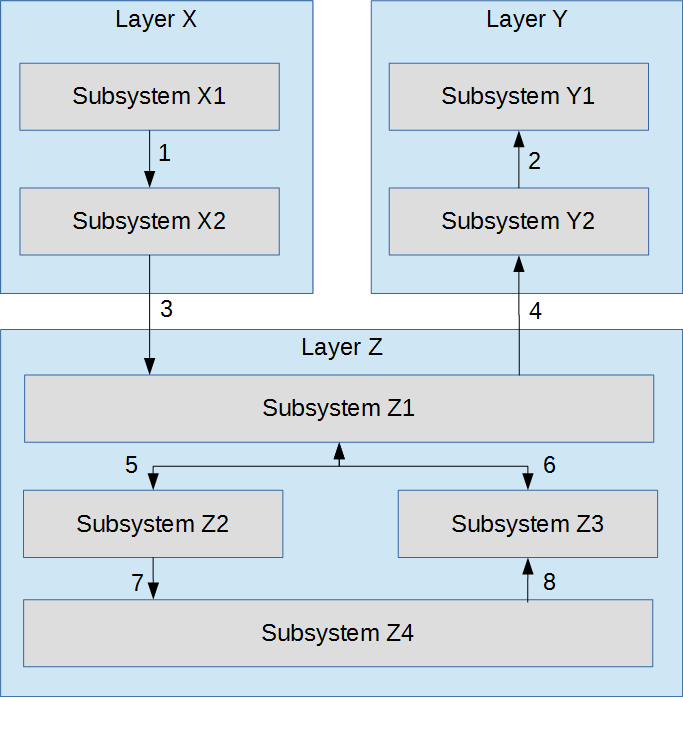
\includegraphics[width=0.90\textwidth]{images/data_flow}
 \caption{System architecture}
\end{figure}

\section{Roles \& Responsibilities}
The sponsor company the team is collaborating with is TrafficNet. Ryan Guadagnolo is the product owner and the main contact from TrafficNet and keeps close contact with Dr. McMurrough and the team. The scrum master is Kyle Edelmann, who ensures that the team is fully functional and productive, while also enabling close cooperation across all roles and functions. The team members are Jose Hernandez, Peyton Casper, Kyle Edelmann, Ruchitha Thalakola, and Rabin Dhaubanjar. The course leader is Dr. Christopher McMurrough, who aids the team in making progress with the project. The only responsibilities each team member has had so far is to finish the project charter tasks that were assigned to each team member. Since the project is at the early stages of development the team does not have concrete roles for each team member. Although some team members like Peyton and Kyle have taken the time to setup the Raspberry Pi which the team will need to begin testing. Once the team has the necessary materials and has everything setup to begin building the project, the team will begin assigning roles to each team member.

\section{Facilities \& Equipment}
The team meetings, development, and testing will be conducted at Senior Design Lab and FAB Lab, where all team members have access to different types of tools. Some of the equipment that will be utilized for this project are a Raspberry Pi, Raspberry Pi camera, infrared camera, surface mount, Axis 214, stepper motors, solar panels, zoom lens, and battery. Since the project is at early stages of development the equipment might change.

\section{Cost Proposal}
\subsection{Preliminary Budget}
The University of Arlington is giving us an inital budget of $800.

\subsection{Current \& Pending Support}
TrafficNet has sponosred our project and pledged an additional $2500.

\section{Documentation \& Reporting}
Lorem ipsum dolor sit amet, quidam omnesque ea vis. Eum an aliquip legendos recusabo. Mea ex purto natum, ne movet fuisset sit. Labore audiam eos ad, facer ornatus posidonium ne ius, et eos duis delenit nusquam.

\subsection{Project Charter}
The project charter will be based off a SBRI and inform readers of the different aspects of the project. It will cover the details of project background information, cost proposals, team structure, sprint planning, individual status reports, engineering notebooks, and deliverables.

\subsection{Product Backlog}
The Product backlog will include any features that need to be finished at some point in the future. Any new features get added to the backlog and transferred to the sprint backlog at the start of the sprint.

\subsection{Sprint Planning}
Spring planning is detail description of the task that the team members will be doing in a whole sprint cycle. The planning will include goal for a certain period which is usually two weeks, backlog that need to be completed in the cycle is discussed and task breakdown between the team members is done. 

\subsubsection{Sprint Goal}
The sprint goal is the list of the tasks that need to be completed during the sprint cycle. There will be different goals for different spring cycle. Every member of the team will be familiar with the sprint goal.

\subsubsection{Sprint Backlog}
The sprint backlog is a list of tasks that are decided in the sprint meeting and that are to completed during the sprint cycle. The tasks are chosen from the product backlog. The team members keep track of the sprint backlog, which also indicates the progress of the project.

\subsubsection{Task Breakdown}
After the backlog has been decided the tasks are divided between the scrum team members. The division of the task is done in such a way that it will help the scrum team member to meet the sprint goal in timely manner. The main goal of the task breakdown is to break a complex task into simpler and smaller tasks.

\subsection{Sprint Burndown Charts}
Sprint burn down chart is the chart that represents a progress during the sprint cycle. The scrum team is required to have a sprint burn down chart after completion of sprint cycle. This charts will show if the scrum team members are utilizing enough time on the tasks or not. The chart contains an estimated time to complete tasks and actual time spend on those tasks.

\begin{figure}[h!]
    \centering
    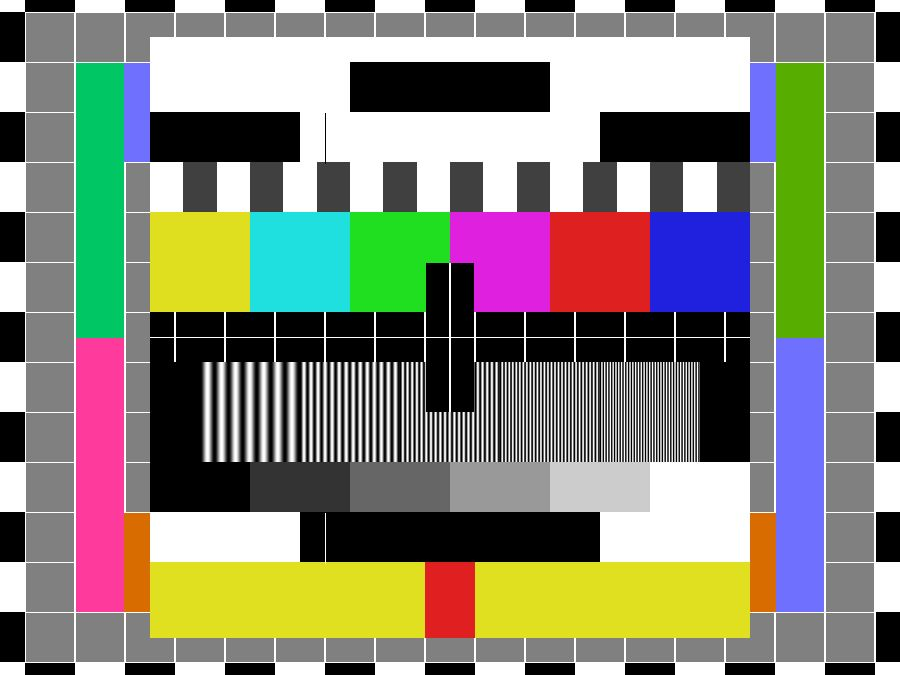
\includegraphics[width=0.5\textwidth]{images/test_image}
    \caption{Example sprint burndown chart}
\end{figure}

\subsection{Sprint Retrospective}
Sprint retrospective is done after every sprint in which whole team participate and discuss about what is working and what is not working. Sprint retrospective is a last thing to work on after completion of the sprint cycle. Things that need to be improved are discussed during the meeting. Product owner, scrum members and scrum master take part in the meeting. 

\subsection{Individual Status Reports}
All the members are required to have this report at the end of the sprint cycle. The main goal of this report is to keep track of team members. In this report team members have to include task they have completed along with time, they have spent and the task they will be working on. Scrum team members are also supposed to include if any other unexpected task appear while completing the given task.

\subsection{Engineering Notebooks}
Engineering notebooks will be used by all team members to record ideas, observations, designs, progress, and what was discussed in team meetings. In addition, the engineering notebook represents official documentation that could be used for patent activities or legal issues. 

\subsection{Closeout Materials}
All the members are required to have this report at the end of the sprint cycle. The main goal of this report is to keep track of team members. In this report team members have to include task they have completed along with time, they have spent and the task they will be working on. Scrum team members are also supposed to include if any other unexpected task appear while completing the given task.

\subsubsection{System Prototype}
The system prototype will consist of a raspberry pi, raspberry pi camera board, pan and tilt motor and brackets, day and night lens, and zoom lens. All of these components will be connected and arranged in an enclosure. 

\subsubsection{Project Poster}
The project poster will contain information regarding the project’s vision, mission, background, and the finished product’s hardware and software details. The poster will be presented at the conclusion of Computer System Design Project II in August, 2016. 

\subsubsection{Web Page}
A web page will be presented to allow the user to view the stream from the camera in a secured manner. They will be allowed to have access with a valid login, password, and IP address. 

\subsubsection{Demo Video}
A demo video will be provided to show how to appropriately use and manage the camera and the software. It will demonstrate all the features of the camera, explain how to view the stream, and describe how to customize the settings in order to fit the needs of the user. The demo video will be delivered through a USB. 

\subsubsection{Source Code}
The source code will consist of software of the user interface to utilize and control the camera. In addition, the source code to allow the user to view the stream of the camera will be provided.  The source code will be delivered in a USB. 

\subsubsection{Source Code Documentation}
The provided source code will be documented properly by including comprehensive comments to allow TrafficNet LLC or their customers to maintain and evolve the software efficiently. The source code documentation will be delivered in a USB. 

\subsubsection{Hardware Schematics}
The design files for the circuit board will be provided to display what was customized in order to attain the appropriate board for the camera. This will be delivered in a USB.

\subsubsection{CAD files}
The CAD files will be provided for any custom made components that are developed. The files will be delivered in a USB. 

\subsubsection{Installation Scripts}
The installation scripts of the web page and the firmware for the camera will be provided. The scripts will be delivered in a USB. 

\subsubsection{User Manual}
A user manual will be provided to describe how to properly operate the camera and utilize the software. It will explain in detail the purpose of each feature of the camera and how to appropriately use them. In addition, the manual will describe the software interface and how to make changes according to the user’s preferences. This will be delivered in a USB. 



\newpage

%%% References
\bibliographystyle{plain}
\bibliographystyle{reference/IEEEtran_custom}
\bibliography{reference/refs}{}

\end{document}